\documentclass[12pt,a4paper]{scrartcl}

\usepackage[a4paper, left=2cm, right=1cm, bottom=1cm, top=1cm, includeheadfoot]{geometry}
\usepackage[ngerman]{babel}
\usepackage[utf8]{inputenc} % comment this if you uncomment utf8x
%\usepackage[utf8x]{inputenc} % uncomment this if there are problems with 'ä', 'ü', 'ö'
\usepackage{ucs}
\usepackage[usenames,dvipsnames]{xcolor}
\usepackage[fleqn]{amsmath}
\usepackage{amsfonts}
\usepackage{amssymb}
\usepackage{color}
\usepackage{listings}
\usepackage{hyperref}
\usepackage{amsfonts}
\usepackage{scrpage2}
\usepackage{graphicx}
\usepackage{pdfpages}
\usepackage{titleps}
\usepackage{lipsum}
\usepackage{textpos}
\usepackage{setspace}
\usepackage{trfsigns}

\newpagestyle{mystyle}{
\sethead[][][]{\name}{\matnr}{\grp}
\setfoot[][][]{\Title}{\thepage}{\sem}
}

\definecolor{mygray}{rgb}{0.9,0.9,0.9}
\lstset{language=[Visual]Basic, morekeywords={param, local}}


\lstset{
   literate={ö}{{\"o}}1
           {ä}{{\"a}}1
           {ü}{{\"u}}1
           {ß}{{\ss}}1
           {é}{{\'e}}1,
   inputencoding=ansinew,
   extendedchars=true,
   basicstyle=\scriptsize\ttfamily,
   numberstyle=\scriptsize,
   breaklines=true,
   tabsize=2,
   numbersep=5pt
}
\lstdefinestyle{customcpp}{
   language=C++,
   backgroundcolor=\color{mygray},
   numbers=left,
   keywordstyle=\color{blue}\bfseries,
   stringstyle=\color{BrickRed}\ttfamily,
   commentstyle=\color{OliveGreen}\ttfamily,
   showspaces=false,
   showstringspaces=false,
   showtabs=false
}
\lstdefinestyle{customoutput}{
   backgroundcolor=\color{mygray},
   numbers=none,
   showspaces=false,
   showtabs=false
}

\newcommand{\sourceCode}[1]{\lstinputlisting[style=customcpp]{#1}}
\newcommand{\tab}{\hspace{20px}}
 %beinhaltet alle benötigten Packages etc.

\pagestyle{mystyle}

%\author{David Kahlbacher - 1619002043}
\title{}

\makeatletter
\newcommand\name{David Kahlbacher 1619002043}
\newcommand\matnr{}
\newcommand\grp{CarrerAI}
\newcommand\sem{}
\let\Title\@title
\makeatother

\begin{document}

%\title{SDP - Uebung 5} % Übungsname und Nummer angeben
%\subtitle{Wintersemester 2014/15} % Semester angeben oder auskommentieren, falls nicht erwünscht
%\author{David Kahlbacher - S1619002043} % Autorenname
%\date{\today}
%\date{} % Das heutige Datum automatisch einfügen

%\maketitle % Titelseite erstellen

\section{Radius Calculation}
To calculate the Radius out of the bowrange and the angle (endpoint angle -- starting angle) the basic equation~\ref{eq:peri} for calculating the perimeter of a circle was settled as starting point. Equation~\ref{eq:radi} shows the final result of the formula transformations.
\begin{flalign}
U &= 2\cdot r\cdot \pi && && && U\ ...\ \text{perimeter}\label{eq:peri}\\
\frac{U}{l} &= \frac{2\cdot r\cdot \pi}{\phi\cdot r} &&\Rightarrow && U = 2\cdot l\cdot \frac{\pi}{\phi}  && r\ ...\ \text{radius}\\
2\cdot l\cdot \frac{\pi}{\phi} &= 2\cdot r\cdot \pi && && && l\ ...\ \text{radian measure}\\
r &= \frac{l}{\phi} && && && \phi\ ...\ \text{angle}
\label{eq:radi}
\end{flalign}

To calculate the angle it is essential to differentiate between left and right curve:
\begin{description}
    \itemsep-2pt
    \item[left:] angle $=$\ output\_angle $-$\ input\_angle
    \item[right:] angle $=$\ input\_angle $-$\ output\_angle
\end{description}

\section{End Point Calculation}
The next formula transformations will show how the endpoint coordinates are calculated in all three cases (left curve, right curve and straight track).\\
Since every track piece exactly has one radius, it can be seen as an equiliteral triangle. The euqiliteral sides have the length of radius $r$, which calculation is shown in equation~\ref{eq:radi}.\\
To calculate the difference between starting point and endpoint the sine and cosine functions will be used. So in addition to the length of the track between start and end point there is a need for the angle of that track. For any straight trails equation~\ref{eq:straightx} and equation~\ref{eq:straighty} can be used. Since it is a straight trail, the input angle and the output angle are the same.

\begin{flalign}
x_{end} &= x_{begin} + l\cdot \cos{(\phi_{in})} \label{eq:straightx}\\
y_{end} &= y_{begin} + l\cdot \sin{(\phi_{in})}\label{eq:straighty}
\end{flalign}

For the slightly more complicated calculation of the end point of a curve first of all the coordinates of the center of the radius circle was calculated (as sort of reference point). To get a better idea of how this formulas come together have a look at figure~\ref{fig:curve_left}.\\
Sine and cosine roles are switched due to the fact that the input and output angles are relative to the negative y-axis. So there is a rotation of $\frac{\pi}{2}$

\begin{flalign}
x_R &= x_{begin} - r\cdot \sin{(\phi_{in})}\\
y_R &= y_{begin} + r\cdot \cos{(\phi_{in})}
\end{flalign}

Starting from this point and the help of the out angle the relative distance between radius center and endpoint can be calculated. The result of the left curve is shown in equation~\ref{eq:leftx} and equation~\ref{eq:lefty}

\begin{flalign}
x_{end} &= x_{R} + r\cdot \sin{(\phi_{out})}\\
y_{end} &= y_{R} - r\cdot \cos{(\phi_{out})}\\
x_{end} &= x_{begin} + r\cdot\left(\sin{(\phi_{out})} - \sin{(\phi_{in})}\right) \label{eq:leftx}\\
y_{end} &= y_{begin} + r\cdot\left(\cos{(\phi_{in})} - \cos{(\phi_{out})}\right)\label{eq:lefty}
\end{flalign}

If we want to calculate the right curve just invert the $+$\ sign in front of $r$. This is shown in equation~\ref{eq:rightx} and equation~\ref{eq:righty}. To get a better idea of why this difference appears have a look at figure~\ref{fig:curve_right}

\begin{flalign}
x_{end} &= x_{begin} - r\cdot\left(\sin{(\phi_{out})} - \sin{(\phi_{in})}\right) \label{eq:rightx}\\
y_{end} &= y_{begin} - r\cdot\left(\cos{(\phi_{in})} - \cos{(\phi_{out})}\right)\label{eq:righty}
\end{flalign}

\begin{figure}
\begin{minipage}{0.45\textwidth}
    \centering
    \includegraphics[width=0.4\textwidth]{LeftCurve}
    \caption{Left curve as a track piece}
    \label{fig:curve_left}
\end{minipage}
\begin{minipage}{0.1\textwidth}
    \centering
    \phantom{}\ \ 
\end{minipage}
\begin{minipage}{0.45\textwidth}
    \centering
    \includegraphics[width=0.36\textwidth]{RightCurve}
    \caption{Right curve as a track piece}
    \label{fig:curve_right}
\end{minipage}
\end{figure}

\section{car flip simulation}

This requires to calculate the centrifugal and the friction force. If the centrifugal force gets greater than the friction force the car will get thrown out of the track. Since the AI is going to receive values from the gyro sensor, we need to transfer the calculated force to the corresponding sensor values. This will be one of the inputs for the AI.

\begin{flalign}
F_R &= m\cdot g\cdot \mu && F_R\ ...\ \text{friction force}
\end{flalign}

For calculating the friction force we have some constant values. $m$\ represents the mass of the car, $g$\ is the gravitational acceleration and $\mu$\ describes the friction coefficient. $\mu$\ could take on different values on different places of the track but this is a possible extension for future use. For easier calculation it will be determined a constant.

An additional problem appears if the wheels are spinning through. In this case the friction coefficient will change (it gets more tiny). There are cases in which just one wheel spins through, or two wheels. In these cases the friction force has to be calculated a little bit more complicated.

\begin{flalign}
F_{Rs} &= g\cdot \sum\limits_{i=1}^4 \left( m_i\cdot {\mu}_i\right) && F_{Rs}\ ...\ \text{friction force spin through} 
\end{flalign}


Since there are 4 wheels we need to calculate the mass for each wheel seperated . The coefficient can take on 2 different values:
\begin{enumerate}
    \itemsep0pt
    \item spin through value
    \item normal spin value
\end{enumerate}

\begin{flalign}
F_Z &= m\cdot r\cdot \omega^2 && F_Z\ ...\ \text{centrifugal force}\label{eq:centri_force}\\
\omega &= \frac{v}{r} && \omega\ ...\ \text{angular speed}\\
v &= n\cdot d_w && v\ ...\ \text{speed of car}
\end{flalign}

The centrifugal force calculates as shown in equation~\ref{eq:centri_force}. The parameter $r$\ describes the radius of the curve which was calculated in equation~\ref{eq:radi}, $n$\ is the rotational speed of the wheels and $d_w$ represents the diameter of the wheels. With these two forces calculated the last step is to differentiate them like $F_R - F_Z$. If the result is positiv the car is still on the planned track, otherwise it will flip out of the track.

\section{gyro sensor}

The gyro sensor consists of 3 values, which represent a rotation in each of the 3 dimensions we know. The mathematical dependencies between $\omega$\ and the gyro rotation around the z -- axis is defined as follows.

\begin{flalign}
Z_{gyro} = a\cdot \omega && Z_{gyro}\ ...\ \text{gyro rotation around z-axis}
\end{flalign}

The parameter $a$\ represents a constant factor which is the difference between $\omega$\ and $Z_{gyro}$. In fig.~\ref{fig:forces} you can see which force shows in which direction. In addition there is an axis of abscissas so you know where the z-axis shows to (for $Z_{gyro}$).

\begin{figure}
    \centering
    \includegraphics[width=0.34\textwidth]{forces}
    \caption{forces in a curve}
    \label{fig:forces}
\end{figure}



\end{document}